\section{Decomposition Rate with Respect to Dominant Fungi Traits}\label{sec:rate}

In this problem, the \textbf{hyphal extension rate} and \textbf{moisture tolerance} are the two basic dominating traits we need to consider in modeling the decay ability of the fungi community.

\subsection{Decomposition  rate model regarding  hyphal  extension  rate,  moisturetolerance and competitive ranking}


\begin{figure}
    \centering
    \begin{minipage}[t]{0.48\textwidth}
        \centering
        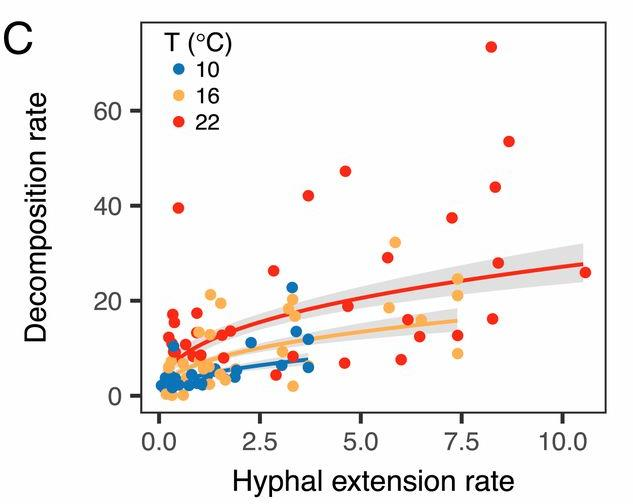
\includegraphics[width=0.8\textwidth]{figure1.jpg}
        \caption{The relationship between the hyphal extension rate (mm/day) of various fungi and the resulting wood decomposition rate (\% mass loss over 122 days) at various temperatures.}\label{fig:hyphal}
    \end{minipage}
    \begin{minipage}[t]{0.48\textwidth}
        \centering
        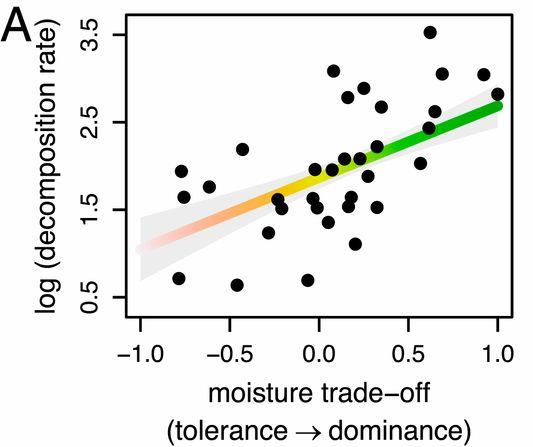
\includegraphics[width=0.8\textwidth]{figure2.jpg}
        \caption{The relationship between the moisture tolerance (difference of each isolate’s competitive ranking and their moisture niche width, both scaled to $[0,1]$) of various fungi and the resulting wood decomposition rate (\% mass loss over 122 days, log transformed).}\label{fig:moisture}
    \end{minipage}
\end{figure}
    

From Figure \ref{fig:hyphal} and Figure \ref{fig:moisture}, it is observed that the relation between the decomposition rate and hyphal extension rate, as well as between the log transformed decomposition rate and relative moisture tolerance are approximately linear.

\begin{equation}
    \left\{\begin{aligned} &
        D = k_1r + b_1 \\ &
        \ln D = k_2(c - m) + b_2
    \end{aligned}\right.
\end{equation}

Apparently, if the hyphal extension rate is $0$, the composition rate would also be $0$, hence the parameter $b_1$ is intrinsically $0$. The model is further specified as

\begin{equation}\label{eq:decay-ability}
    \left\{\begin{aligned} &
        D = k_1r \\ &
        \ln D = k_2(c - m) + b_2.
    \end{aligned}\right.
\end{equation}

% TODO: tolerance, ranking, width?

Note that, in \ref{fig:moisture}, the $x$-axis variable is not exactly the moisture tolerance (moisture niche width), instead is the difference of each isolate’s competitive ranking and their moisture niche width, in range $[-1, 1]$. Hence in the model, competitive ranking $c$ is taken into consideration.


\subsection{Decomposition rate data fitting for single fungus isolate}

Based on the traits data of various species of fungus provided in [], and the resulting experimental 

The fitting result is shown below



% TODO: cite the references, and label where the data comes from

\subsection{Extending the model to multi-species system}

\begin{figure}\label{fig:community}
    \begin{minipage}{0.4\textwidth}
        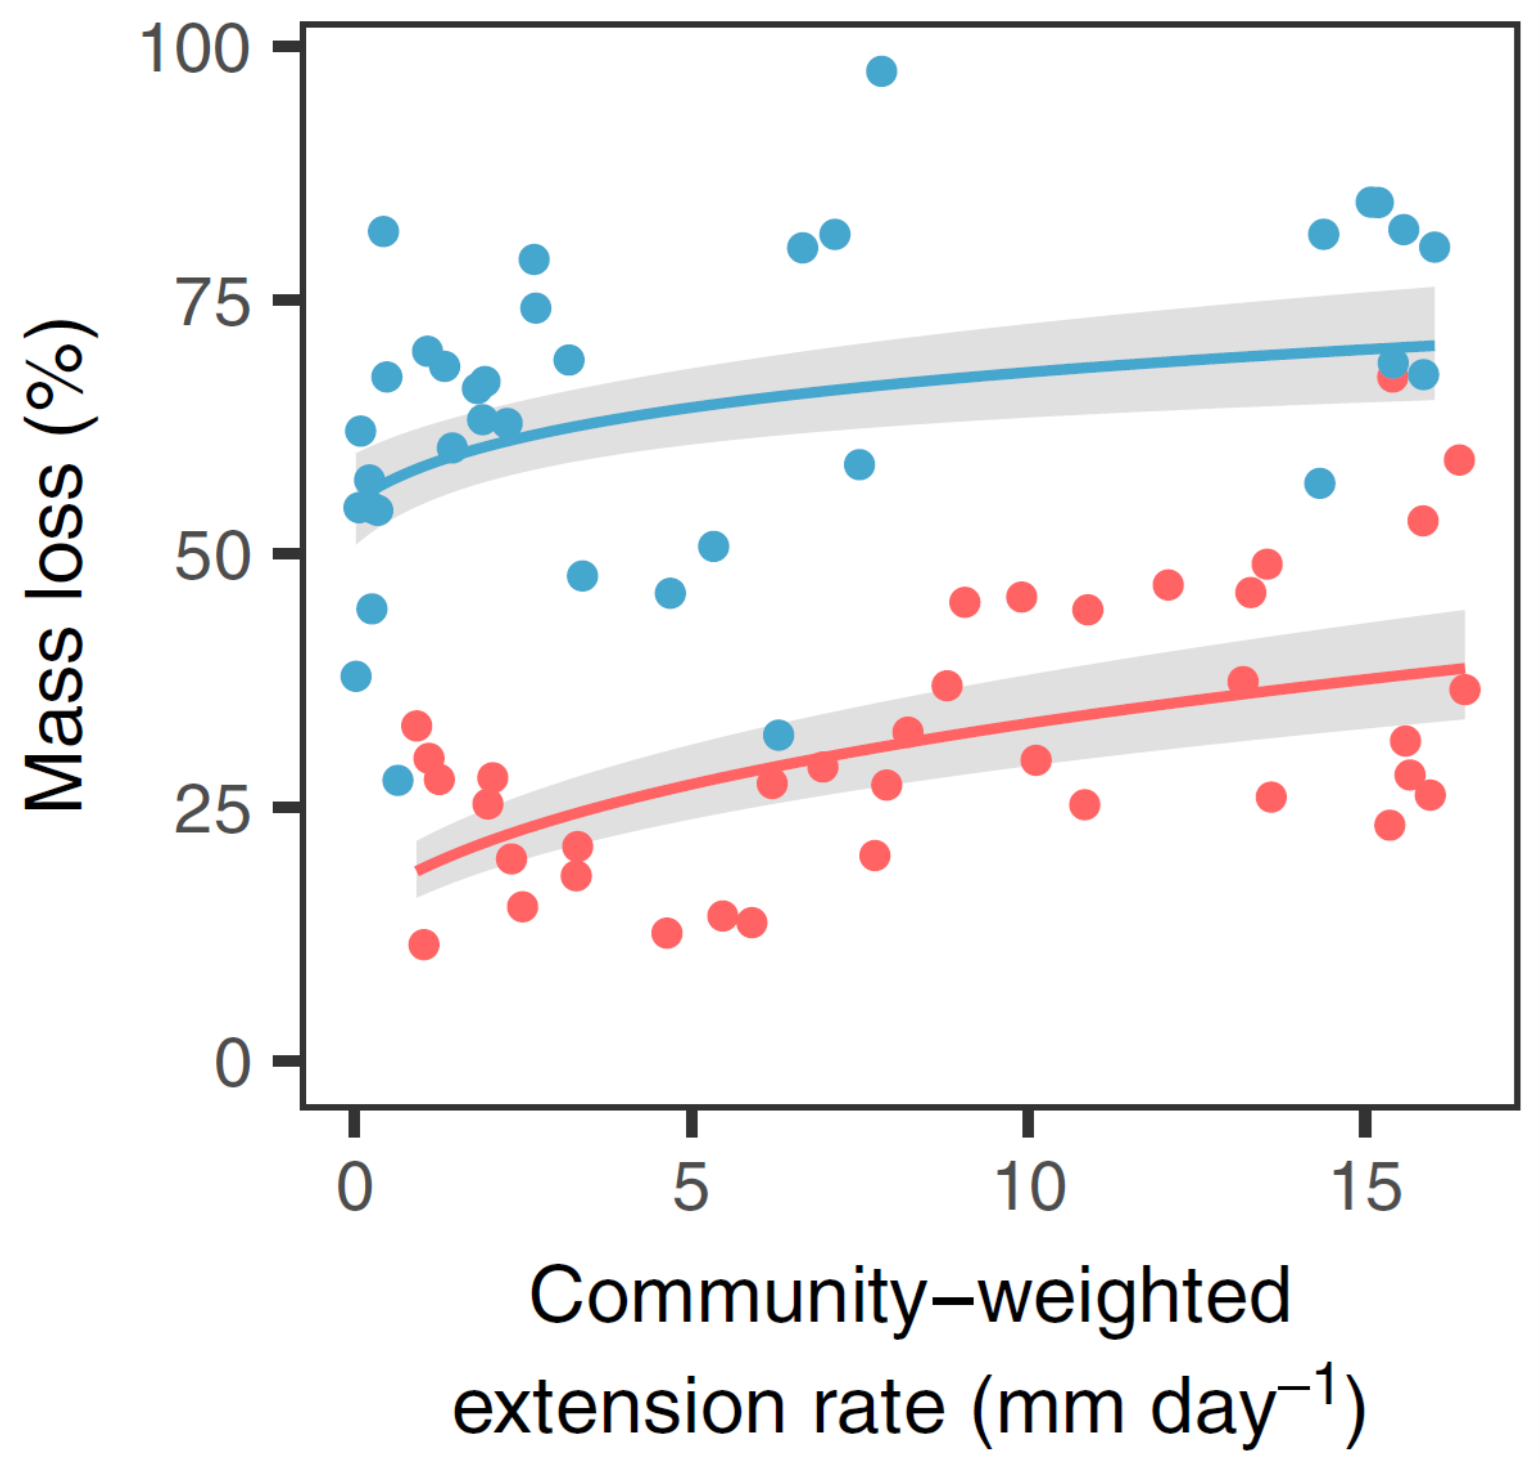
\includegraphics[width=\textwidth]{figure3.png}
    \end{minipage}
    \begin{minipage}{0.5\textwidth}
        \caption{The decomposition of logs increases with the hyphal extension rate of the fungal community that colonized them. This figure is adapted from []}
    \end{minipage}
\end{figure}

For multi-species case, according to [], the decomposition of logs increases with the hyphal extension rate of the community, and is approximately characterized by a linear model with respect to the community-weighted mean extension rate. Therefore, in order to describe the decay ability of a community consists of multiple species of fungus, the relative quantity relation between of each isolate in the community is necessary.

The decay ability of a fungi community can be described quantitatively as the following expression.

\begin{equation}\label{eq:dcomm}
    D_\text{comm} =
    k_3\bar{r} =
    k_3\frac{r_1x_1 + \cdots + r_nx_n}{x_1 + \cdots + x_n} =
    k_3\dfrac{\sum_{i=1}^n r_ix_i}{\sum_{i=1}^n x_i}.
\end{equation}

% TODO: cite the references, and label where the data comes from

With the data presented in [], the coefficient $k_3$ is roughly determined as [] for 3 years of decay, [] for 5 years. 

% TODO: relation with time

Research conducted in [] presents the data obtained from experimental results on various wood substrate for 3 years or 5 years.

For solving this model for practical prediction of the decay ability of fungi community, each $x_i$ needs to be specified. This part is discussed in the following sections.
